
\subsubsection{Introduction}
This chapter evaluates the best, average and worst cases for the Ullman and the VF2 algorithms in
terms of time and memory efficiency. The best, average and worst cases are by the graph traver-
sal stratedy that is followed by both algorithms as well as the number of edges that the graphs have.\newline\newline
The best, average and worst cases for graph matching are define below as well as a graphical representation of 10 vertices 
depicting how the specific case looks like.

\textbf{Best case:} The best case for graph matching G A onto graph G B is defined as a graph G A having
no edges defined in their graphs, i.e $E$ {\tiny A} = 0. Figure \ref{fig:best_case} depicts a graph of 10 vertices depicting the
best case scenario.

\begin{figure}[H]
  \begin{center}
      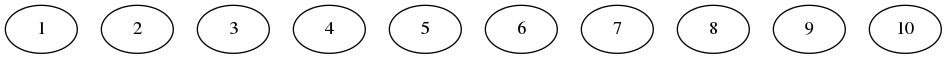
\includegraphics[width=0.8\textwidth]{best.png}
  \end{center}    
  \caption{Graph of 10 vertices representing the best case scenario}
  \label{fig:best_case}
\end{figure}

\textbf{Average case:} The average case for graph matching $G$ {\tiny A} onto $G$ {\tiny B} is defined as a graph $G$ {\tiny A} with
half of its vertices connected to each other. Thus the graph will have $(n(n − 1)/2)/2$ edges that are uniquily connected to each vertice in 
the graph. Figure \ref{fig:average_case} depicts a graph of 10 vertices depicting the average case scenario.

\begin{figure}[H]
  \begin{center}
      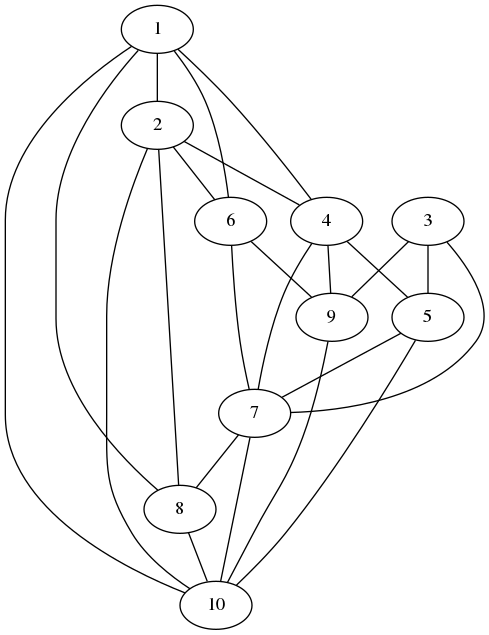
\includegraphics[width=0.4\textwidth]{average.png}
  \end{center}    
  \caption{Graph of 10 vertices representing the average case scenario}
  \label{fig:average_case}
\end{figure}

\textbf{Worst case:} The worst case for matching graph $G${\tiny A} onto $G${\tiny B} is defined as a graph $G${\tiny A} with all its vertices connected
to eact other. Thus the graph will have $n(n − 1)/2$ edges that are uniquily connected to each vertice in the graph. Figure \ref{fig:worst_case} depicts
a graph of 10 vertices depicting the worst case scenario.

\begin{figure}[H]
  \begin{center}
      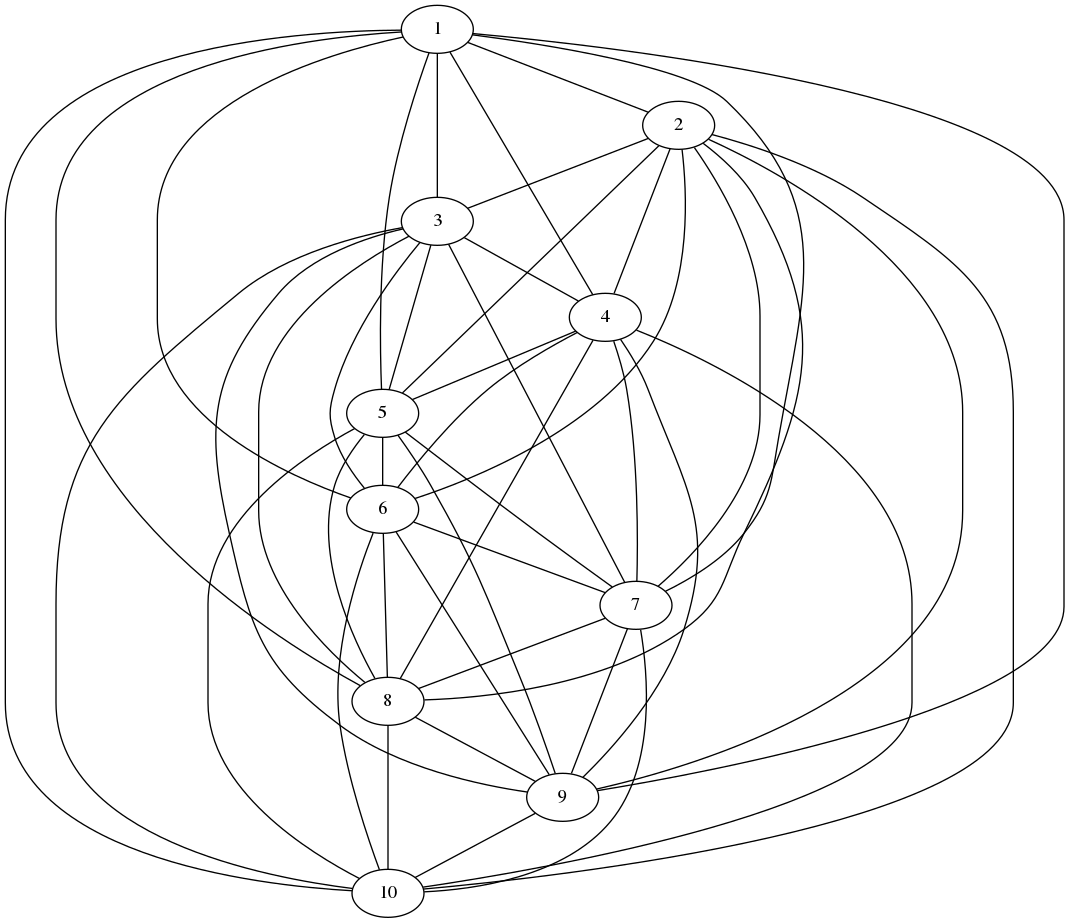
\includegraphics[width=0.5\textwidth]{worst.png}
  \end{center}    
  \caption{Graph of 10 vertices representing the worst case scenario}
  \label{fig:worst_case}
\end{figure}